\section{Fungal growth}

The life cycle of filamentous microorganisms typically begins and ends as a spore, which are produced from the microbe's fruiting bodies and dispersed by air, water, or possibly by animals. The spore will usually remain dormant until the necessary environmental conditions for activation are met, but how this dormancy is maintained is poorly understood. There is evidence that low levels of metabolic activity are necessary to maintain spore viability; O\sb{2} consumption and CO\sb{2} production by \emph{Neurospora} ascospores were found to be 1 -- 4\% that of vegetative cells \cite{carlile2001}. However, prolonged viability has been demonstrated in the absence of metabolism; fungi have been grown from glacial ice cores estimated to be up to 140,000 years old \cite{carlile2001}.

Various physical agents, such as light, temperature and chemical compounds, can cause activation of fungal spores \cite{tauro1986}. Of most importance however is the availability of water and a minimum water activity\footnote{$a_w$; ratio of vapour pressure of water in a substance to the vapour pressure of pure water at the same temperature} of approximately 0.65 is required for growth of most fungi \cite{walker2005}. The germination rate of \emph{P. chrysogenum} spores has been demonstrated to be highly dependent on water activity \cite{sautour2001}, while both temperature and water activity were shown to be significant in determining the germination rate of \emph{Aspergillus ochraceus} spores \cite{pardo2005}. Some microbes may also require nitrogen or carbon sources for spore activation \cite{medwid1984}, while others can germinate in pure water, the growth being supported by endogenous reserves \cite{carlile2001}. Large numbers of spores in close proximity may fail to germinate (self-inhibition); in some species, the frequency of germination increases as the concentration of spores is decreased \cite{moore-landecker1996}. Some species require a \lq trigger', such as heat or chemical stimulus, that may not necessarily be required to maintain vegetative growth, to initiate spore germination. For example, exposure to temperatures of 50 -- \celc{60} for approximately 20~minutes is required by ascospores of \emph{Neurospora} to initiate germination \cite{moore-landecker1996}. Germinative potential has implications for industrial processes, as variations in the number of viable spores in the inoculum can have a considerable influence on the outcome of a fermentation (Section~\ref{sec:InocConc}).

Once the conditions for activation have been met, spores undergo a swelling process, during which their size may increase up to four-fold due to the uptake of water \cite{robson1999}. Trinci reported that during the first 4~hours after inoculation, \emph{Rhizopus stolonifer} sporangiospores increased linearly in diameter \cite{trinci1971a}. In their analysis of the development of \emph{A. oryzae}, Spohr and colleagues found that the spores remained approximately spherical during enlargement, although it was difficult to differentiate between exponential growth in the spore volume and a linear increase in the spore equivalent diameter \cite{spohr1998}. The swelling process culminates in the emergence of one or more germ tubes from the spore, the extension rate of which increases exponentially until a constant rate is attained \cite{trinci1971a}, which varies between species and is also dependent on the prevailing environmental conditions. The extension of the germ tube ($q_{germ}$) may be described by the following empirical, Monod-type expression \cite{spohr1998}:

\begin{equation}\label{eq:qgerm}
	q_{germ} = k_{germ} \ . \ \frac{l_{germ}}{l_{germ} + K_{germ}}
\end{equation}

\noindent where $k_{germ}$ is the maximum extension rate and $K_{germ}$ is a saturation constant. Alternatively, the length of the germ tube ($l_{germ}$) at time $t$ is given as follows \cite{prosser1995}:

\begin{equation}
	l_{germ} = \left \{ \begin{array}{l l}	l_0 e^{k_1 t} & t \leq t_l\\
																				l_l + k_2 t & t > t_l\end{array} \right .
\end{equation}

\noindent where $k_1$ and $k_2$ are constants, $t_l$ represents a point in time when $l_{germ} >> K_{germ}$ ($\therefore q_{germ} \approx k_{germ}$) and $l_0$ and $l_l$ are germ tube lengths at $t=0$ and $t=t_l$ respectively. Such empirical kinetic expressions are generally based on experimental data, with little or no knowledge of the underlying growth mechanisms. This is as opposed to mechanistic models, which are typically more complex to enable quantitative consideration of assumptions on growth \cite{prosser1995}.

Extension of the germ tube, or hypha, is confined to the apical region; extension occurring in sub-apical regions would result in \lq buckling' and distortion of the hypha. Early studies of this mechanism involved \lq dusting' sub-apical hyphal regions with particles and noting any displacement of these particles over time as the growth of the organism proceeded; those particles that adhered to hyphae did not alter their position \cite{carlile2001}. Apical advancement is a result of internal hydrostatic pressure within the hypha forcing the thin, plastic apical cell wall outward; hyphae contain high concentrations of solutes, resulting in water entering the cells by osmosis and generating positive turgor pressure \cite{gow1995}. As growth proceeds, the cell wall in sub-apical regions becomes thicker, more rigid and more resistant to turgor pressure \cite{ruiz-herrera1991}, restricting hyphal growth to the apical region. The advancement of apical cells often occurs at the direct expense of cytoplasm in sub-apical cells, resulting in the formation of vacuoles, which are typically not seen in the proximity of hyphal tips \cite{paul1998}. The cell wall formation driving hyphal extension is a vesicle-based process, with the vesicles\footnote{A vesicle is a sac that stores or transports substances intra-cellularly} (containing the precursors required for cell wall formation) believed to be supplied by the Vesicle Supply Centre (VSC) \cite{bartnicki-garcia1989}, also known as the apical body or Spitzenk\"{o}rper. The VSC, visible under phase-contrast microscopy as a dark region located just behind an advancing hyphal tip, has been implicated in \lq guiding' hyphal growth. The formation of a new branch is preceded by the formation of a new Spitzenk\"{o}rper, while a change in direction in hyphal growth is preceded by a displacement of the apical body \cite{carlile2001}.

In the higher fungi, internal cross-walls termed septae are formed at regular intervals as the hypha extends, sub-dividing the hypha into individual cells. In the event that a breach of the cell wall occurs, the pores within these septae are \lq plugged', so that loss of cytoplasm is confined to one particular cellular compartment and death of the entire hypha does not occur. It has been demonstrated that cutting a sub-apical compartment does not result in the death of the apical cell, although a reduction in extension rate may be observed \cite{trinci1971}.

When a hypha has attained a certain length, a branch is formed laterally to the parent, typically towards the end of the period of exponential extension \cite{trinci1974,prosser1995}. An expression similar to Equation~(\ref{eq:qgerm}) may be used to describe the extension of branches, but the value of the saturation constant, $K_i$, may vary significantly within a single mycelium; there is evidence suggesting $K_i$ is proportional to the distance between a newly-formed branch and the tip of the \lq primary' hypha \cite{spohr1998}. The process of branching is poorly understood, although a correlation with septation has been proposed, as branches often form just behind septae \cite{carlile2001}. It has been postulated that a hypha will produce a branch if the material supply to a hypha exceeds that required for the maintenance of growth of a single hypha, or, when transport of material distant from the tip becomes limited. This may be explained by the formation of a septum behind the advancing tip, after which extension is dependent on biosynthesis within the apical region \cite{prosser1995}. Branches are typically formed in acropetal succession behind the primary tip, with the formation of a new branch preceded by a softening of the rigid sub-apical cell wall at the location where the new branch emerges \cite{moore-landecker1996}.

The critical branch length that results in a new branch being spawned is referred to as the hyphal growth unit ($\hgu$), which is approximately equal to the total hyphal length ($\Lh$) divided by the total number of tips ($N$) on any given element. First proposed by Plomley \cite{plomley1959}, this represents the mean length of hypha required to support tip growth. If mycelial growth involves the duplication of a \lq growth unit', it follows that $\Lh$ and $N$ increase exponentially at approximately the same specific growth rate. That is, branching attains an exponential rate, with each individual branch growing at approximately the same linear rate, resulting in a similar exponential increase in biomass. This was first demonstrated experimentally by Trinci in a study of \emph{Neurospora crassa}, \emph{Aspergillus nidulans}, \emph{Geotrichum candidum}, \emph{Mucor hiemalis} and \emph{P. chrysogenum} \cite{trinci1974}. Colonies were cultivated on cellophane-covered media (to restrict growth to two dimensions) and measures of the dimensions were made on enlarged photographic prints. After an initial period of discontinuous branch production, exponential growth was observed (Fig.~\ref{fig:Fig1Trinci1974}), although a wide variation in the growth rate of individual branches was noted. Measured specific growth rates varied from approximately \h{0.25} for \emph{A. nidulans} up to \h{0.60} for \emph{M. hiemalis}. The growth unit was also studied in batch cultures of \emph{G. candidum} by Caldwell and Trinci, who reported that total hyphal length and the number of branches per mycelium increased exponentially with biomass, suggesting that the ratio of total mycelium to number of tips was constant \cite{caldwell1973}. Furthermore, it was found that the hyphal growth unit remained relatively constant for specific growth rates ranging from 0.173 to \h{0.385}, supporting the hypothesis that the mould had a functional unit of hyphal growth.

\begin{figure}[t]
	\centering
	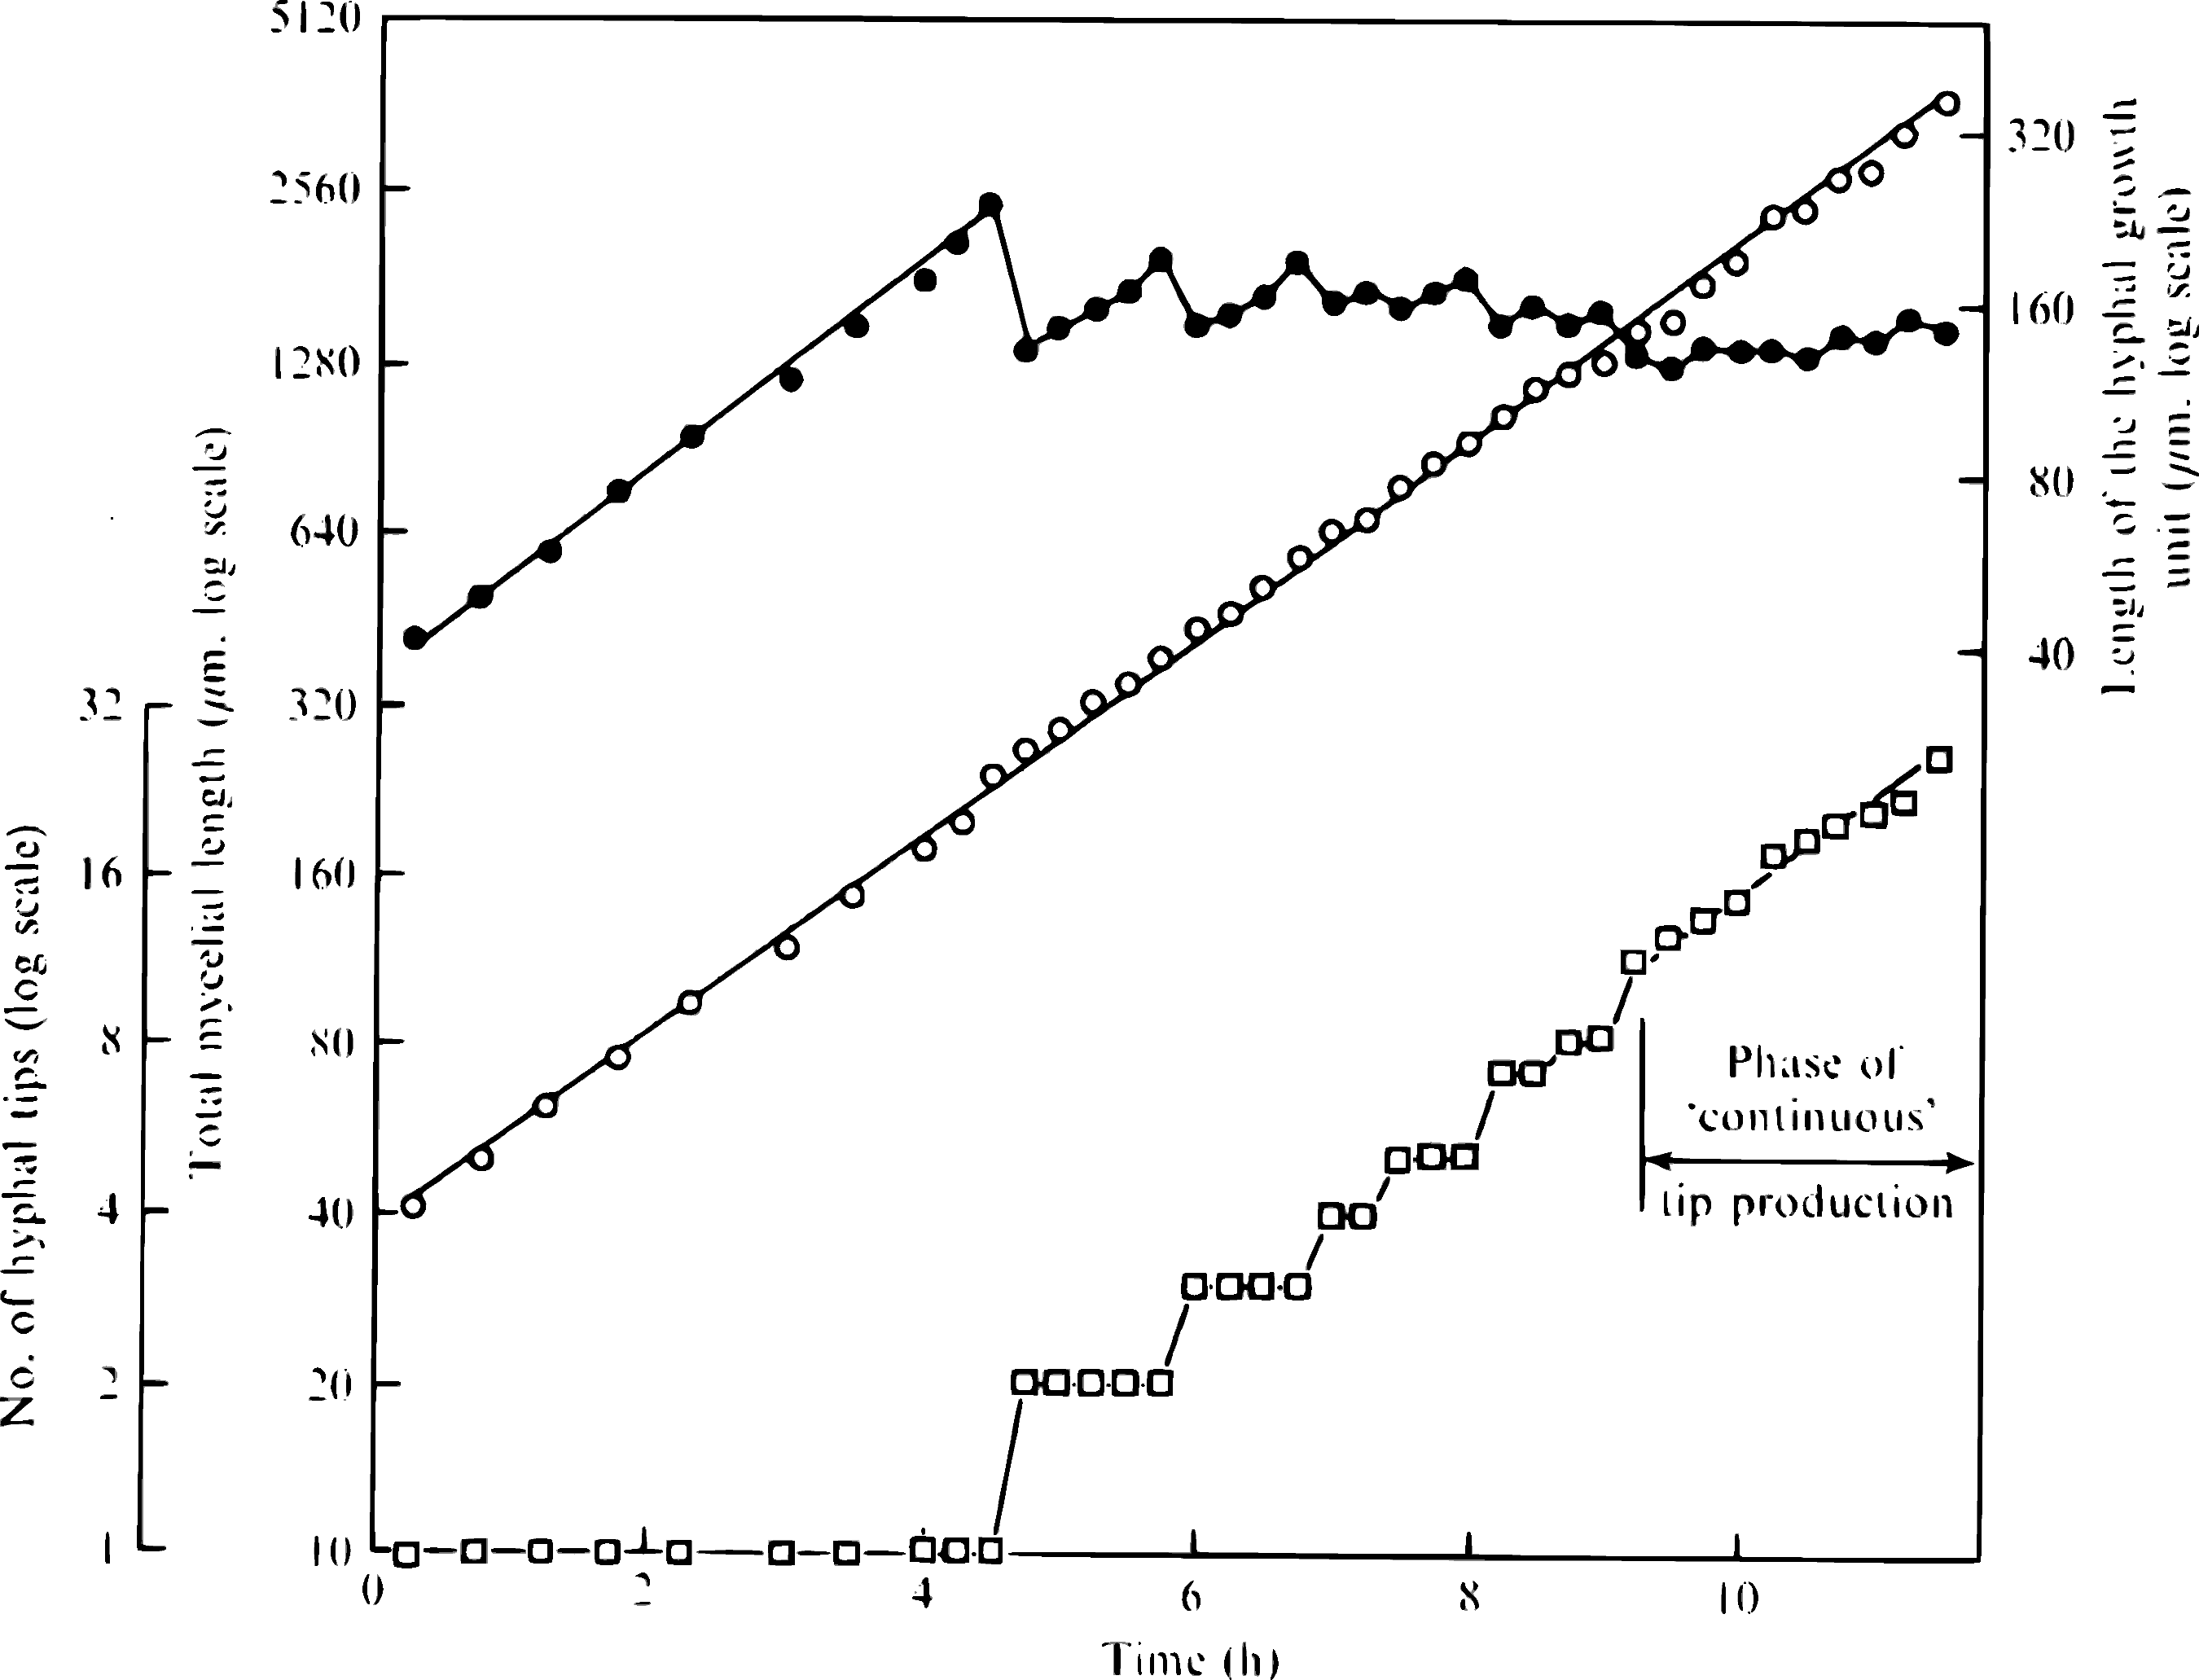
\includegraphics[width=(\textwidth - 1cm)]{../C1/Fig1Trinci1974}
	\caption{Growth of a mycelium of \emph{Geotrichum candidum} on solid medium, as described by Trinci \cite{trinci1974}, showing number of tips ($\Box$), total hyphal length ($\circ$) and hyphal growth unit ($\bullet$). Reproduced with permission from the Society for General Microbiology.}
	\label{fig:Fig1Trinci1974}
\end{figure}

In young mycelia exhibiting undifferentiated growth, the mean rate of hyphal extension ($E$; \h{\omic~tip\sp{-1}}) may be calculated as follows \cite{prosser1995}:

\begin{equation}\label{eq:ELN}
	E = \frac{2(\Lh - \Lho)}{N_t + N_0}
\end{equation}

\noindent where $\Lho$ and $\Lh$ are the total hyphal lengths at time $t=0$ and 1~hour later, while $N_0$ and $N_t$ are the respective number of hyphal tips. The mean extension rate may then be related to the specific growth rate ($\mu$; \oh) as follows:

\begin{equation}
	E = \mu \hgu
\end{equation}

\noindent Over time, nutrient limitations will arise at the centre of the colony, where germination occurred, eventually resulting in the cessation of growth at this location (and often sporulation occurs) \cite{prosser1995}. A differentiated colony is thus formed, in which growth is restricted to the colony periphery, where abundant nutrients are still available. The active region is referred to as the peripheral growth zone, the width of which ($w$) may be determined by modifying the formula proposed by Trinci \cite{trinci1971}:

\begin{equation}
	w = \frac{K_r}{\mu}
\end{equation}

\noindent where $K_r$ is the radial expansion rate of the colony (\omich). Alternatively, if an estimate for $w$ is known, then $\mu$ may be calculated by measuring the change in colony radius over time. However, such an approach would not take into consideration aerial hyphae or hyphae growing into media substrata \cite{moore-landecker1996}. Furthermore, variations in the direction of growth of individual hyphae will affect their contribution to radial extension \cite{prosser1995}.

Growth in such a manner results in the formation of a \lq sink', into which nutrients diffuse, and a \lq source', from which metabolites effuse, and, consequently, concentration gradients develop within the medium. An analysis conducted by Olsson showed graphically that such gradients existed in medium supporting the growth of \emph{Fusarium oxysporum} colonies \cite{olsson1994}, with a particularly steep decline in glucose and phosphate concentration at the colony edge, while the concentration of both nutrients was virtually zero at the colony centre. Radially-directed growth away from the colony centre is probably a consequence of such gradients \cite{carlile2001}, but the mechanism by which fungi grow in such patterns, efficiently exploiting the available substrate, is not fully understood. The tendency of hyphae to avoid each other is particularly evident at the edge of a colony, where branches are formed at acute angles, and may be a response to a signalling metabolite secreted by the hyphae themselves (autotropism) or a localised depletion of oxygen (or higher concentration of carbon dioxide) around the hyphae (chemotropism) \cite{robson1999}.

\subsection{Growth in submerged batch culture}

In a closed, \lq batch' system, a volume of media is inoculated and growth proceeds until the concentration of an essential nutrient becomes limiting, or toxic compounds have reached a critical, growth-inhibiting level. A stationary liquid culture will result in the formation of a fungal \lq mat' on the media surface. Agitation results in the formation of submerged culture, in which the growth form varies between a homogeneous suspension of dispersed hyphae and discrete pellets (Fig.~\ref{fig:LifeCycle}). Non-septate organisms typically grow poorly in such environments, as the shear forces caused by agitation result in excessive loss of cytoplasm from cells.

The early stages of growth of filamentous microbes in submerged liquid culture are similar to those described above for an undifferentiated mycelium. The growth is well described using kinetic equations derived from unicellular bacterial studies, such that biomass, substrate and product are assumed to be uniformly distributed \cite{prosser1995}. Following an initial lag phase\footnote{If the fermentation was inoculated with an exponentially-growing culture, growth continues exponentially and no lag phase occurs}, during which the organism acclimatises to a new environment after inoculation, branching attains an exponential rate. The rate of change of biomass ($x$) may therefore be described as:

\begin{equation}
	 \frac{dx}{dt} = \mu x 
\end{equation}

\noindent Integrating yields:

\begin{equation}
	 \ln x_t = \ln x_0 + \mu t 
\end{equation}

\noindent where $x_t$ is the level of biomass at time $t$ and $x_0$ is biomass at time $t=0$. This equation may also be written as:

\begin{equation}
	 x_t = x_0 \ e^{\mu t} 
\end{equation}

\noindent This growth phase, following the initial lag, is thus termed the exponential growth phase (Fig.~\ref{fig:GrowthPhases}) and will continue as long as the necessary environmental conditions to support it exist (nutrients in excess, adequate aeration, favourable temperature and pH). In industry, this growth phase is of interest for the production of biomass and growth-associated metabolites, such as amylases, cellulases and proteases, which are typically required for the synthesis of nutrients. The secretion of these metabolites can be influenced by the media composition, as the production of certain enzymes may be induced by the presence of a particular substrate. Furthermore, if a mixture of sugars is present in the medium, low-molecular weight substrates, such as glucose in particular, will typically be preferentially consumed by the organism. This is typically achieved by the inhibition (or repression) of the synthesis of enzymes involved in the catabolism of other carbon sources (known as catabolite repression) \cite{moore-landecker1996}.

\begin{figure}[t]
	\centering
	\pstool[width=10.5cm]{../C1/GrowthPhases}{
		\psfrag{x}[Bc]{\al $\ln x$}
		\psfrag{t}[Bc]{\al Time}
		\psfrag{L}[Bl]{\al Lag}
		\psfrag{l}[Bl]{\al Phase}
		\psfrag{E}[Bl]{\al Exponential}
		\psfrag{e}[Bl]{\al Phase}
		\psfrag{S}[Bl]{\al Stationary}
		\psfrag{s}[Bl]{\al Phase}}
  \caption{Typical growth profile of a microorganism grown in submerged culture, where $x$ denotes biomass.}
  \label{fig:GrowthPhases}
\end{figure}

The specific growth rate attained during the exponential phase is dependent on nutrient concentration; if all nutrients required for growth are present in excess, then the specific growth rate attains a maximal value ($\mu_{max}$). The empirical relationship between $\mu$ and nutrient concentration ($s$) may be expressed in terms of Monod kinetics (Fig.~\ref{fig:Monod}):

\begin{equation}
	 \mu = \mu_{max} . \frac{s}{s + K_s} 
\end{equation}

\noindent where $K_s$ is a saturation constant, which is typically very small relative to the concentration of the relevant nutrient in the media. As such, in a laboratory environment in which a chemically-defined medium is used, all nutrients will typically be present in amounts vastly greater than the respective saturation constants and the specific growth rate will approximate $\mu_{max}$ during the exponential phase.

%While most fungi are capable of both aerobic and anaerobic metabolism, the absence of oxygen typically results in much lower growth rates, but most can grow in poorly aerated conditions as the saturation constant ($K_s$) for oxygen can be very low (0.1\% v/v for \emph{A. oryzae} \cite{rahardjo2005b}). Essential for growth is some form of carbon source, the simplest of which, glucose, is usable by virtually all fungi \cite{carlile2001}. However, many fungi are capable of degrading polysaccharides such as starch, cellulose and chitin. The availability of nitrogen can also limit growth.  As is the case with spore activation, a high water potential is required by most microbes for hyphal growth. The inability of fungi to grow in the absence of water is the basis for food preservation techniques such as drying or curing with salt. The prevailing temperature typically has a significant impact on the growth rate of fungi. Although most fungi can growth over a relatively broad range of temperatures (typically a few degrees above 0\sp{o} up to 30~-~40\sp{o}C), most have an optimal value at which the specific growth rate is maximal.

\begin{figure}[t]
	\centering
	\pstool[width=10.5cm]{../C1/Monod}{
		\psfrag{g}[Bc]{\al $\mu$ (\oh)}
		\psfrag{s}[Bc]{\al $s$}
		\psfrag{k}[Bl]{\al $K_s$}
		\psfrag{m}[Bl]{\al $\mu_{max}$}
		\psfrag{n}[Bl]{\al $\mu_{max}/2$}}
  \caption{Specific growth rate ($\mu$) versus nutrient concentration ($s$) according to Monod kinetics. Half of the maximum specific growth rate ($\mu_{max}$) is attained when $s$ is equal to the saturation constant $K_s$.} 
  \label{fig:Monod}
\end{figure}

The exponential growth phase is ended as a result of the exhaustion of a nutrient required for growth or the accumulation of growth-inhibiting compounds. The culture then enters the stationary phase of growth, the transition involving substantial physiological changes, which again, may be influenced by media composition. During the stationary phase, cell growth is balanced by cell death, but compounds of industrial interest, such as organic acids, vitamins and lipids, may be accumulated in the culture. A fourth growth phase, termed the decline phase, may follow the stationary phase, during which cell growth is outpaced by cell death and biomass declines as a result.

An important variant of the batch culture format is \lq fed-batch culture', in which biomass is initially grown in a batch system until a pre-determined point in time, perhaps relating to the exhaustion of a chosen medium component. Fresh nutrient is then added, typically as a concentrated form of a component of the original medium. Conducting fermentations in this manner may be used to, for example, minimise medium viscosity in the event that a starch substrate is employed, or, if glucose is utilised as substrate, to maintain the concentration below repressing levels. The fed-batch format may also be used to add an inducer to initiate secretion of a particular metabolite, or to maintain the limiting nutrient conditions necessary for secondary metabolite production. The majority of large-scale industrial fungal fermentations are of the fed-batch variety.

%\subsubsection{Continuous culture}

%An alternative to the batch culture format is continuous flow culture, in which the exponential phase of growth can be maintained for an extended period of time. Following medium inoculation, further nutrient medium is added to the culture at a constant dilution rate ($D$). Overflow of microorganism and media is collected and the culture volume therefore remains constant. In steady-state operation, a constant level of biomass is maintained in the culture, growing at a constant specific growth rate determined by $D$. While this culture format is useful for physiological studies in the laboratory, it is uncommon in industry.

\subsubsection{Growth in the form of pellets}

Depending on the organism, pellet formation can result from the aggregation of spores prior to germination, aggregation of spores and germ tubes or, less commonly, the aggregation of mycelia \cite{prosser1995}. A wide range of physiochemical parameters may affect the pellet formation process, some of which will be discussed in Section~\ref{sec:ProcVarMorph}.

Pelleted cultures have long been assumed to follow cube root kinetics \cite{emerson1950,marshall1960}:

\begin{equation}
	x^{1/3} = {x_0}^{1/3} + kt
\end{equation}

\noindent where $x$ is biomass at time $t$, $x_0$ is biomass at time $t=0$ and $k$ is a constant.  The growth of fungi in the form of pellets is somewhat analogous to colony growth on solid substrates; over time, growth of the pellet will be restricted to an outer \lq active layer' (the width of which, $w$, is dependent on the diffusional properties of the mycelium \cite{prosser1995}) as the core of the pellet suffers from diffusion limitations \cite{pirt1966}. Changes in the pellet radius may be described by:

\begin{equation}
	r = r_0 + w \mu t
\end{equation}

\noindent If the pellet is assumed to be spherical with a constant biomass density ($\rho$), increase in biomass can be rewritten as follows:

\begin{equation}
	x = x_0 + \left( \frac{4}{3} \pi \rho n \right )^{1/3} w \mu t
\end{equation}

\noindent where $n$ is the number of pellets. Exponential growth is predicted (while $r \leq w$) until restrictions to diffusion of nutrients through the pellet mass reduce growth rates in the centre of the pellets ($r > w$); subsequent growth will then follow cube-root kinetics.

Over time, diffusion limitations will lead to a cessation of biomass production at the pellet core and the onset of autolysis. This leads to a reduction in stability and the pellet becomes more susceptible to damage by mechanical forces. Furthermore, hyphal elements at the pellet surface become weakened by ageing and vacuolation, making them more susceptible to shearing. Consequently, the macroscopic morphology can change considerably \cite{paul1999}. Pellet break-up often results in growth renewal, provided nutrient requirements are met (the medium will be enriched by nutrients from autolysed biomass), since fragments can act as centres for new growth \cite{papagiannireview}. This complex relationship between pellet growth, fragmentation and regrowth has been studied in a variety of organisms (Table~\ref{tab:PelletBatchLit}).

\begin{table}[htbp]
	\centering
	\footnotesize
	\caption{Recent reports in the literature on the development of fungal pellets in batch cultivations.}
	\label{tab:PelletBatchLit}
	\begin{tabularx}{(\textwidth - 1cm)}{l R c}
		\toprule
		Organism & Report & Reference \\ \midrule
		\emph{A. oryzae} & Pellet radius increased linearly up 35 hours before onset of fragmentation & \cite{carlsen1996a}\\
		\emph{A. niger} & Pellet formation completed 15~h post-inoculation - pellets increased in size but not in numbers. Active region of pellets decreased from 20~h & \cite{elenshasy2006}\\
		 \emph{A. terreus} & Pellet size increased up to approximately 75~h and remained relatively constant thereafter in shake-flasks inoculated with pellets, although free mycelia were visible after 120~h & \cite{bizukojc2009}\\
		 \emph{A. niger} & Pellet size increased continuously with cultivation time in shake-flask culture & \cite{papagianni2004}\\
		 \emph{A. niger} & Pellet diameter levelled off between approximately 50 and 100~h cultivation, depending on the inoculum concentration & \cite{papagianni2002}\\
		 \emph{C. militaris} & Pellet size increased over the course of 8-day fermentation, but sucrose concentration was high (40~g/L) & \cite{jppark2002}\\
		 \emph{A. terreus} & Pellets in stirred-tank reactors increased in size before falling in later stages & \cite{rodriguezporcel2005}\\
		 \emph{A. niger} & Approximately 50~hours post-inoculation, a transition from \lq smooth' to \lq hairy' pellets took place, indicated by a decline in fullness ratio (area/convex area) & \cite{paul1998}\\
		 \emph{P. baumii} & Small pellets with filamentous growth changed into \lq feather-like' mycelial clumps. Diameter declined from 5.2 to 2.6~mm after 12~days & \cite{hwang2004}\\
		 \emph{P. gilvus} & Pellets were compact and smooth until latter stages of fermentation when hollow cores formed and diameter declined & \cite{hwang2004}\\
		 \emph{P. linteus} & Pellets exhibited compact central cores with loose filamentous outer zones. Diameter, core area and circularity increased during fermentation & \cite{hwang2004}\\
		\bottomrule
	\end{tabularx}
\end{table}

The growth of \emph{A. oryzae} in the form of pellets was studied in detail by Carlsen and colleagues \cite{carlsen1996a}. In the time period of 18 to 32~hours post-inoculation, the number of pellets was almost constant and the pellet radius increased with a constant rate of \mich{37.5}, which was very similar to the value of \mich{35} reported for the hyphal tip extension rate in freely dispersed cultures. After 35~hours of cultivation, the pellet concentration rapidly increased, whereas the mean pellet radius decreased, but the growth in biomass was described very well by the cube-root law prior to pellet break-up ($t > 35$~h). Thereafter, a smaller fraction of the biomass was mass-transfer limited, resulting in an increase in $\mu$. Oxygen limitation in pellet cores set in approximately 23~hours after inoculation and, after 35~hours, approximately 50\% of the biomass was estimated to be limited by oxygen. The concentration of ethanol in the media was found to increase with the estimated oxygen-limited biomass concentration, while no ethanol production was detected in batch cultivations grown as freely dispersed hyphal elements.